% Created 2021-10-30 Sat 15:54
% Intended LaTeX compiler: pdflatex
\documentclass[11pt]{article}
\usepackage[utf8]{inputenc}
\usepackage[T1]{fontenc}
\usepackage{graphicx}
\usepackage{grffile}
\usepackage{longtable}
\usepackage{wrapfig}
\usepackage{rotating}
\usepackage[normalem]{ulem}
\usepackage{amsmath}
\usepackage{textcomp}
\usepackage{amssymb}
\usepackage{capt-of}
\usepackage{hyperref}
\author{Mari§}
\date{\today}
\title{03}
\hypersetup{
 pdfauthor={Mari§},
 pdftitle={03},
 pdfkeywords={},
 pdfsubject={},
 pdfcreator={Emacs 27.2 (Org mode 9.5)}, 
 pdflang={English}}
\begin{document}

\maketitle
\tableofcontents

\section{Notas:}
\label{sec:org2298a99}
\subsubsection{Cenário X}
\label{sec:orgda0aec6}
\begin{itemize}
\item \textbf{Use case}
\begin{itemize}
\item \textbf{Descrição:}
\item \textbf{Cenário:}
\item \textbf{Pré-condição:}
\item \textbf{Pós-condição:}
\item \textbf{Fluxo normal:}
\item \textbf{Fluxo de excepção:}
\end{itemize}
\end{itemize}

\section{Portagens}
\label{sec:org1fac779}
\subsection{1ª Etapa}
\label{sec:org169ca8c}
Identificar os atores e use case do sistema.
Através de texto, tabelas, \ldots{}

\textbf{Atores:}
\begin{itemize}
\item Cliente
\item Pórtico
\item Gestor
\end{itemize}

\begin{center}
\begin{tabular}{ll}
\hline
\textbf{Ator} & \textbf{Use Case}\\
\hline
\textbf{Cliente} & Pesquisar movimentos\\
 & Listar movimentos\\
 & Obter extrato mensal\\
\hline
\textbf{Pórtico} & Registar passagem do veículo\\
\hline
\textbf{Gestor} & Alterar tabela de preços\\
\hline
\end{tabular}
\end{center}

\subsection{2ª Etapa}
\label{sec:orgd7bcd3c}
(1ª versao) do diagrama U.C

Realizado através do \textbf{Visual Paradgma}
\begin{center}
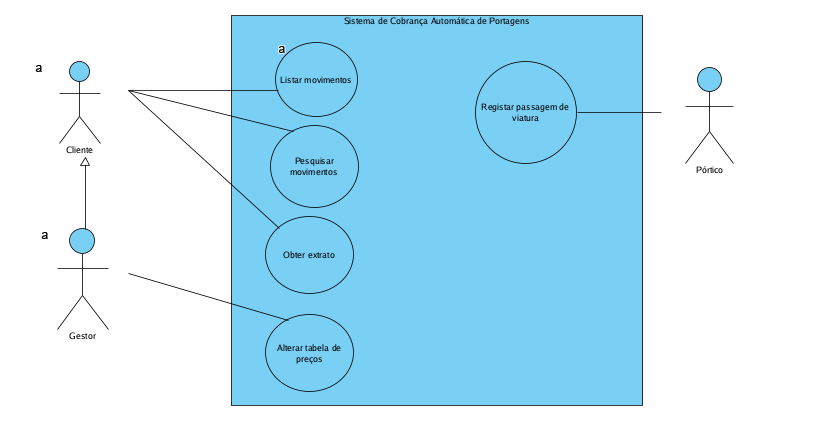
\includegraphics[width=.9\linewidth]{./portagens.png}
\end{center}

\subsection{3ª Etapa}
\label{sec:org2395d5f}
Descrever cada um dos use cases.

\subsubsection{Cenário 1}
\label{sec:org3b0e1fb}
\textbf{Use case} Registar passagem de viatura

\begin{itemize}
\item \textbf{Cenário:}
Cenário 1 -Numa viagem Mindelo-Valença a uzana fez o percurso pela A 28, uma ex-SCUT \ldots{}

\item \textbf{Pré-condição:}
True (Não tem pré-condição).

\item \textbf{Pós-condição:}
O Sistema fica com mais um registo de passagem na  base de dados.

\item \textbf{Fluxo normal:}

\textbf{1.} O pórtico comunica o \textbf{identificador} da viatura (\texttt{e o número pórtico})

\textbf{2.} O Sistema de portagens valida que o identificador encontra-se registado.

\textbf{3.} Cria o registo (\texttt{identificador}, \texttt{hora}, \texttt{local} e o \texttt{número pórtico}).

\item \textbf{Fluxo Alternativo 1} \texttt{[identificador não reconhecido](passo 2)}

\textbf{2.1} O Sistema comunica que o identificador não consta na base de dados.

\textbf{2.2} Pórtico envia fotografia do veículo para posterior análise.

\textbf{2.3} Sistema cria um registo (\texttt{fotografia}, \texttt{identificador}, \texttt{hora}, \texttt{local} e o \texttt{número pórtico}).

\item \textbf{Fluxo Alternativo 2} \texttt{[pórtico não conseguiu ler o identificador](passo 1)}

\textbf{1.1} O Pórtico envia um identificador errado.

\textbf{1.2} O Sistema comunica que o identificador não consta na base de dados.

\textbf{1.3} Pórtico envia fotografia do veículo para posterior análise.

\textbf{1.4} Sistema cria um registo (\texttt{fotografia}, \texttt{identificador}, \texttt{hora}, \texttt{local} e o \texttt{número pórtico}).
\end{itemize}

\section{Biblioteca}
\label{sec:org3630c35}
\subsection{1ª Etapa}
\label{sec:orgeb31b87}
\textbf{Atores:}
\begin{itemize}
\item Utilizador
\item Funcionário
\end{itemize}

\begin{center}
\begin{tabular}{ll}
\hline
\textbf{Ator} & \textbf{Use Case}\\
\hline
\textbf{Utilizador} & Pesquisar um livro\\
 & Requisitar livro\\
\hline
\textbf{Funcionário} & Registar requisição de livro\\
 & Registar devolução de livro\\
 & Renovar a requisição de um livro\\
 & Passar multas???\\
 & \ldots{}\\
\hline
\end{tabular}
\end{center}

\subsection{2ª Etapa}
\label{sec:orgd3df0e6}
Fazer diagrama\ldots{}
\subsection{3ª Etapa}
\label{sec:org8982499}

\subsubsection{Cenário 1}
\label{sec:org1db0939}
\begin{itemize}
\item \textbf{Use case:} Registar requisição de um livro.
\begin{itemize}
\item \textbf{Cenário:}
O josé requisita um dado livro.

\item \textbf{Pré-condição:}
Funcionário encontra-se registado.

\item \textbf{Pós-condição:}
O sistema fica com mais um registo de requisição de um livro.

\item \textbf{Fluxo normal:}

\textbf{1.} Funcionário indica o código do utent e o código do livro.

\textbf{2.} Sistema verifica que o utente é válido.

\textbf{3.} Sistema verifica que o utente não tem multas pra pagar ou se tem livros com entrega em atraso.

\textbf{4.} Sistema verifica disponibilidade do livro.

\textbf{5.} Sistema calcula data prevista de entrega para devolução.

\textbf{6.} Sistema regista requisição do livro pelo utente.o livro pode ser requisitado e atualiza estado do livro em questão.

\textbf{7.} Sistema imprime o comprovativo de requisição

TODO Fazer fluxo de excepção
\item \textbf{Fluxo de excepção:}
\begin{itemize}
\item O utente pode nao existir
\item livro nao tem disponibilidade
\item \ldots{}.
\end{itemize}
\end{itemize}
\end{itemize}
\end{document}
